%This is a XeLaTeX document compile it with xelatex
%OCR: tesseract
%Compile few times to add table of contents
%everything provided in this file and PDF are free to use
%
%Creative Commons Legal Code
%
%CC0 1.0 Universal
%
%    CREATIVE COMMONS CORPORATION IS NOT A LAW FIRM AND DOES NOT PROVIDE
%    LEGAL SERVICES. DISTRIBUTION OF THIS DOCUMENT DOES NOT CREATE AN
%    ATTORNEY-CLIENT RELATIONSHIP. CREATIVE COMMONS PROVIDES THIS
%    INFORMATION ON AN "AS-IS" BASIS. CREATIVE COMMONS MAKES NO WARRANTIES
%    REGARDING THE USE OF THIS DOCUMENT OR THE INFORMATION OR WORKS
%    PROVIDED HEREUNDER, AND DISCLAIMS LIABILITY FOR DAMAGES RESULTING FROM
%    THE USE OF THIS DOCUMENT OR THE INFORMATION OR WORKS PROVIDED
%    HEREUNDER.
%
%Statement of Purpose
%
%The laws of most jurisdictions throughout the world automatically confer
%exclusive Copyright and Related Rights (defined below) upon the creator
%and subsequent owner(s) (each and all, an "owner") of an original work of
%authorship and/or a database (each, a "Work").
%
%Certain owners wish to permanently relinquish those rights to a Work for
%the purpose of contributing to a commons of creative, cultural and
%scientific works ("Commons") that the public can reliably and without fear
%of later claims of infringement build upon, modify, incorporate in other
%works, reuse and redistribute as freely as possible in any form whatsoever
%and for any purposes, including without limitation commercial purposes.
%These owners may contribute to the Commons to promote the ideal of a free
%culture and the further production of creative, cultural and scientific
%works, or to gain reputation or greater distribution for their Work in
%part through the use and efforts of others.
%
%For these and/or other purposes and motivations, and without any
%expectation of additional consideration or compensation, the person
%associating CC0 with a Work (the "Affirmer"), to the extent that he or she
%is an owner of Copyright and Related Rights in the Work, voluntarily
%elects to apply CC0 to the Work and publicly distribute the Work under its
%terms, with knowledge of his or her Copyright and Related Rights in the
%Work and the meaning and intended legal effect of CC0 on those rights.
%
%1. Copyright and Related Rights. A Work made available under CC0 may be
%protected by copyright and related or neighboring rights ("Copyright and
%Related Rights"). Copyright and Related Rights include, but are not
%limited to, the following:
%
%  i. the right to reproduce, adapt, distribute, perform, display,
%     communicate, and translate a Work;
% ii. moral rights retained by the original author(s) and/or performer(s);
%iii. publicity and privacy rights pertaining to a person's image or
%     likeness depicted in a Work;
% iv. rights protecting against unfair competition in regards to a Work,
%     subject to the limitations in paragraph 4(a), below;
%  v. rights protecting the extraction, dissemination, use and reuse of data
%     in a Work;
% vi. database rights (such as those arising under Directive 96/9/EC of the
%     European Parliament and of the Council of 11 March 1996 on the legal
%     protection of databases, and under any national implementation
%     thereof, including any amended or successor version of such
%     directive); and
%vii. other similar, equivalent or corresponding rights throughout the
%     world based on applicable law or treaty, and any national
%     implementations thereof.
%
%2. Waiver. To the greatest extent permitted by, but not in contravention
%of, applicable law, Affirmer hereby overtly, fully, permanently,
%irrevocably and unconditionally waives, abandons, and surrenders all of
%Affirmer's Copyright and Related Rights and associated claims and causes
%of action, whether now known or unknown (including existing as well as
%future claims and causes of action), in the Work (i) in all territories
%worldwide, (ii) for the maximum duration provided by applicable law or
%treaty (including future time extensions), (iii) in any current or future
%medium and for any number of copies, and (iv) for any purpose whatsoever,
%including without limitation commercial, advertising or promotional
%purposes (the "Waiver"). Affirmer makes the Waiver for the benefit of each
%member of the public at large and to the detriment of Affirmer's heirs and
%successors, fully intending that such Waiver shall not be subject to
%revocation, rescission, cancellation, termination, or any other legal or
%equitable action to disrupt the quiet enjoyment of the Work by the public
%as contemplated by Affirmer's express Statement of Purpose.
%
%3. Public License Fallback. Should any part of the Waiver for any reason
%be judged legally invalid or ineffective under applicable law, then the
%Waiver shall be preserved to the maximum extent permitted taking into
%account Affirmer's express Statement of Purpose. In addition, to the
%extent the Waiver is so judged Affirmer hereby grants to each affected
%person a royalty-free, non transferable, non sublicensable, non exclusive,
%irrevocable and unconditional license to exercise Affirmer's Copyright and
%Related Rights in the Work (i) in all territories worldwide, (ii) for the
%maximum duration provided by applicable law or treaty (including future
%time extensions), (iii) in any current or future medium and for any number
%of copies, and (iv) for any purpose whatsoever, including without
%limitation commercial, advertising or promotional purposes (the
%"License"). The License shall be deemed effective as of the date CC0 was
%applied by Affirmer to the Work. Should any part of the License for any
%reason be judged legally invalid or ineffective under applicable law, such
%partial invalidity or ineffectiveness shall not invalidate the remainder
%of the License, and in such case Affirmer hereby affirms that he or she
%will not (i) exercise any of his or her remaining Copyright and Related
%Rights in the Work or (ii) assert any associated claims and causes of
%action with respect to the Work, in either case contrary to Affirmer's
%express Statement of Purpose.
%
%4. Limitations and Disclaimers.
%
% a. No trademark or patent rights held by Affirmer are waived, abandoned,
%    surrendered, licensed or otherwise affected by this document.
% b. Affirmer offers the Work as-is and makes no representations or
%    warranties of any kind concerning the Work, express, implied,
%    statutory or otherwise, including without limitation warranties of
%    title, merchantability, fitness for a particular purpose, non
%    infringement, or the absence of latent or other defects, accuracy, or
%    the present or absence of errors, whether or not discoverable, all to
%    the greatest extent permissible under applicable law.
% c. Affirmer disclaims responsibility for clearing rights of other persons
%    that may apply to the Work or any use thereof, including without
%    limitation any person's Copyright and Related Rights in the Work.
%    Further, Affirmer disclaims responsibility for obtaining any necessary
%    consents, permissions or other rights required for any use of the
%    Work.
% d. Affirmer understands and acknowledges that Creative Commons is not a
%    party to this document and has no duty or obligation with respect to
%    this CC0 or use of the Work.

\documentclass[11pt, twoside, finnish, a5paper]{book}
\usepackage[
    type={CC},
    modifier={zero},
    version={1.0},
]{doclicense}

\usepackage[utf8]{inputenc}
\usepackage{amsmath}
\usepackage{amsfonts}
\usepackage{amssymb}
\usepackage{lmodern}
\usepackage[a5paper]{geometry}
\usepackage[finnish]{babel}
\usepackage{titlesec}
\usepackage{hyperref}
\usepackage{fontspec}
\usepackage{eso-pic}
\usepackage{graphicx}
\usepackage[xetex]{attachfile2}
\usepackage{xcolor}
\usepackage{bookmark}

\hypersetup{
  pdftitle={Ihmistuntija},
  pdfauthor={Robert Tunning},
  pdfsubject={Physiognomy},
  pdfproducer={Otto Andersin Oy. Kirjapaino Pori, 1937},
  pdfcreator={pdflatex},
  pdfstartview={FitBH},
}

\setmainfont{Crimson Text}

\AddToShipoutPictureBG{%
  \AtPageLowerLeft{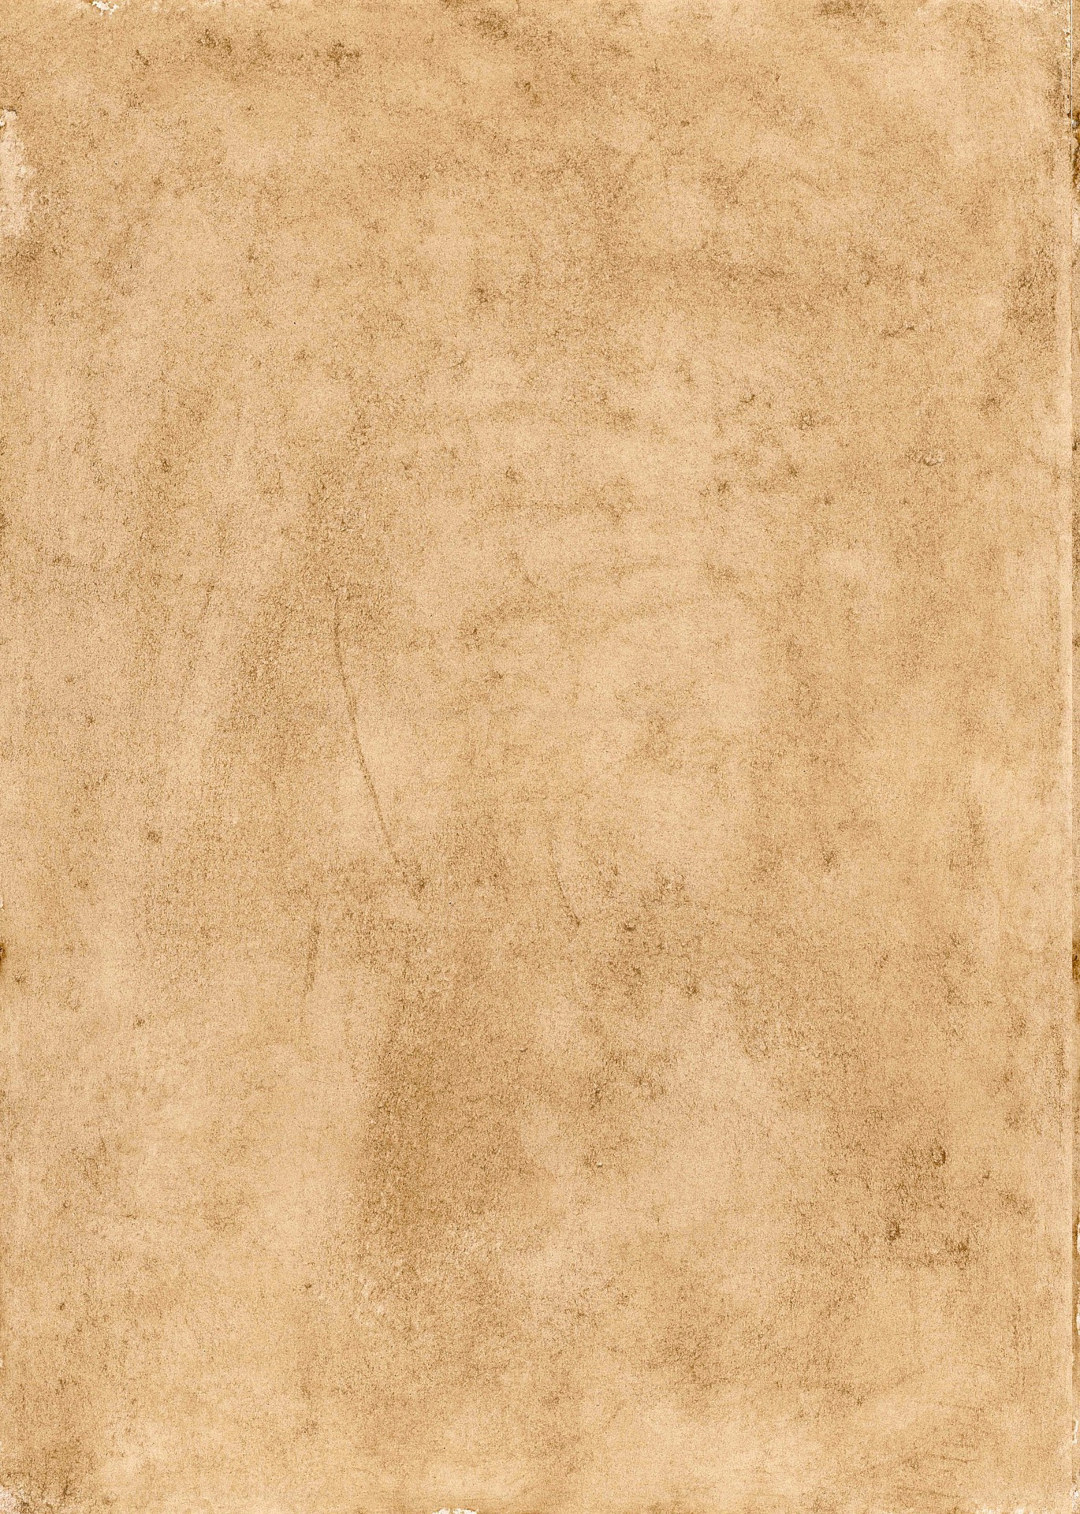
\includegraphics[width=\paperwidth,height=\paperheight]{old.jpg}}%
}


\titleformat{\paragraph}[block]{\fontspec{Crimson Text}\bfseries\centering}{\theparagraph}{1em}{}[]
\titlespacing*{\paragraph}{0pt}{\baselineskip}{0pt}

\titleformat{\chapter}[display]
  {\Huge\bfseries}
  {\filcenter\fontsize{50}{60}\fontspec{Crimson Text}\selectfont\thechapter}
  {1ex}
  {\filcenter\fontsize{25}{30}\bfseries}
\fontspec{Crimson Text}

\author{Toht. Robert Tunning}
\title{Ihmistuntija}
\date{1937}
 
\begin{document}
\begin{titlepage}
    \centering
    {\Huge\bfseries IHMISTUNTIJA\par}
    \vspace{3cm}
	\textbf{ tahi taito, että ensimmäisestä silmäyksestä erehtymättä
voi arvostella niiden henkilöiden luonnetta, taipumuksia,
elämän tapoja j.n.e., joiden kanssa elämässä tulemme
yhteyteen.}

 \vspace{1cm}
 
 {\large \textbf{ Aikamme välttämättömin}\par}
 
  \vspace{0.1cm}

    {\Large \textbf{ Käsikirja}\par}
    
      \vspace{0.1cm}

\textbf{ kaikille niille, jotka ulkonaisesta ihmisestä
tahtovat tulla tuntemaan sisällisen.}
    
    \vfill
    {\large Kirjoitti\par}
    {\Large \textbf{ Toht. Robert Tunning}\par}
    \vspace{1cm}
    %{\large 1937\par}

    
    {\Large \textbf{ Otto Andersin Oy. Kirjapaino Pori, 1937}\par}
        {\large \textit{Kirjanen on kuvaluettu ja teksitunnistettu suomennoksesta}}
    \textattachfile[description=Ei toimi välttämättä kaikilla lukijoilla, author=Robert Tunning]{ihmistuntija.tex}{\textcolor{black}{\footnotesize{\textbf{Tallenna kirjasen lähdekoodi}}}}
\textattachfile[description=Ei toimi välttämättä kaikilla lukijoilla, author=Robert Tunning]{old.jpg}{\phantom{.}}

\end{titlepage}

\tableofcontents
\markboth{}{}
\begingroup

\titleformat{\chapter}[display]
  {\Huge\bfseries}
  {\filcenter\fontsize{50}{60}\fontspec{Kleist Fraktur}\selectfont\thechapter}
  {1ex}
  {\filcenter\fontsize{25}{30}\bfseries}
\
\fontspec{Kleist-Fraktur} 


\chapter*{Johdanto.} 
\addcontentsline{toc}{chapter}{Johdanto}

Meille ihmisille ei ole mikään tarpeellisempi ja hyödyllisempi 
kuin ihmistuntemus, ja kuitenkin ovat niin
harvat ne, jotka ovat hankkineet itselleen tarkemman ja
syvemmän tiedon siinä taidossa, että ulkomuodosta ja
tavallisessa kanssakäymisessä oikein voisivat tuntea,
mikä ihminen on, mitä hän ajattelee, toivoo ja tahtoo.
Moni matkustaa maat ja kaupungit, joutuu 
kanssakäymiseen monien ihmisten kanssa, oppii niin tuntemaan
heidän sovinnoiset elämäntapansa ja luulee nyt olevansa
ihmistuntemuksen syvimmissä salaisuuksissa. — Mutta
mitä hän tietää ihmisistä?
Nämä näyttävät hyviksi ulkonaisen olentonsa puolesta,
juuri kun puettuna pyhävaatteisiinsa, mutta sentään ovat
itserakkauden ja omanvoiton orjat. — Ja tätä hän nimittää
ihmistuntemiseksi.— Miksi ihmiset näin menettelevät, eikä toisin;
miksi on heidän ajatuksillansa ja käytöksillänsä
tällainen muoto? Siitä vähän väliä! Hän osaa vaistomaisesti käyttää
itsensä heitä kohtaan ja he häntä, ja molemmat
koettavat saavuttaa tarkoituksensa niin paljon kuin
mahdollista.

Tällainen varjomainen ihmistunteminen ei kuitenkaan
ole riittävä, vaikka ihan tavallinen, mutta meidän pitää tunkea
syvemmälle ja tuoda ilmi ilmauksen syyt. Meidän ei pidä
pysähtymän pinnalle, vaan tunkea siitä niihin salaisiin konepajoihin,
joissa ajatukset syntyvät, taipumukset ja tahto muodostuvat,
halut ja päätökset lähtevät ja joista kaiken elämän
ja toimen peruslähde saa alkunsa.

Joka perinpohjin tahtoo oppia tuntemaan ihmisiä,
hänen täytyy sitä ennen tulla tuntemaan itsensä, hänen
täytyy tietää mitkä sielunvoimat ihmisellä on, kuinka
nämä vaikuttavat, mihinkä ne pyrkivät ja kuinka ne
osittain sotivat toinen toistansa vastaan, osittain
sopusoinnussa käyvät määrättyyn maaliinsa. Se joka tuntee
itsensä, se voi tuntea myös muita ja käyttää sen hyödyksensä.
Salaisuudessa, jossa kiihoittimet vaikuttavat,
havaitsee hän sen, mitä muut ajattelevat ja tahtovat.

Yhdellä on suurempi päättämiskyky tahi älykkyys
kuin toisella. Hän ymmärtää teeskennellä ja saavuttaa
viekkaudella tarkoituksensa, jonka kolmas 
voittaa rehellisyydellä.

Mailmassa näyttäytyy ihminen sellaisena kun hän
— näkee itsellensä olevan hyödyksi. Usein peittää joku
tekopyhäisellä vanhurskaudella viekkaan sydämensä,
usein salaa suuri omanvoiton pyytäjä tahi konna ja
pettäjä vikansa rehellisyyden ja ihmisyyden varjolla. —
Mutta silloin on ihmistuntijan katsominen verhon läpi
ja tunteminen teeskentelijä, voidaksensa varustautua
hänen paheitansa vastaan ja oikein käyttää itsensä
häntä kohtaan.

Miten tämä on mahdollista ilmoitetaan seuraavissa lehdissä.
\endgroup



\begingroup

\chapter*{Yleinen ruumiin muodostus.}
\addcontentsline{toc}{chapter}{Yleinen ruumiin muodostus}

Jos kohta ei yleisestä ruumiin muodosta voida saada
niin vakavia päätöksiä ihmisen sisällisestä olennosta kuin
kasvoista, niin on edellinen kumminkin sangen tärkeä
ihmistuntijalle, varsinkin sentähden kun ruumis ei salli
teeskentelemistä, niinkuin kasvot. Ruumiin kasvanto
ja sen suhde, mikä on sen erityisten osain välillä,
vaikuttavat sangen paljon ihmisen älylliseen ja siveelliseen
luonteeseen. Sen, joka tahtoo tulla tuntemaan ihmisen
sisällistä olentoa, täytyy huomioonsa ottaa myös yleinen
ulkonaisen ruumiin muoto ja sen erityiset osat.

Koska ihmisen ruumiilla on yhtähyvin fysiognomiansa
(kasvotietonsa) kuin kasvoillakin, niin saakoon muutamat
katselmukset yleisestä ruumiin rakennuksesta tässä tilansa.

Että täydellinen sopusointu on ihmisen ruumiin ja mielenlaadun
välillä, näemme siitä, jos vertaamme lihavan
laihaan, suuren vähäiseen, epäsäännöllisen säännölliseen ihmiseen.

Koska lihavalla ihmisellä on aina taipumus laiskuuteen,
hitaisuuteen tahi hiljaisuuteen, niin on laihalla taas sitä
vastaan aina enemmän tahi vähemmän ärtyinen, äkkinäinen,
rauhaton ja elävä luonne. Suuressa ihmisessä näemme
vakavuutta ja lujuutta, mutta pienessä yleisesti
kevytmielisyyttä ja välinpitämättömyyttä. Koska säännöllinen
ruumis, useimmissa tapauksissa, on juuri kuin jalouden
juuri eli peruste, niin voimme olla vakuutetut siitä,
että epäsäännöllinen on heikkouden eli heikon sielun asunto.

Sielu, joka, niinkuin tiedämme, on ihmisen kaikkein
toimintain, päätöksien, taipumuksien ja tunteiden lähde,
ilmoittaa se aina itsensä näkyväisesti.
Siihen, että tahtonsa voimalla peittää
sielunsa todellisia tunteita ja taipumuksia,
on jokaisen ihmisen pyrkiminen, niin paljon
kuin mahdollista. Vaan jos tämä menestyykin muutamassa
kohden, etenkin silloin, kun tutkija on harjaantumaton
fysiognomiassa, niin ei ole kuitenkaan teeskenteleminen
mahdollinen oikian ihmistuntijan edessä, joka
arvostelee ja päättää kokonaisuuden mukaan.

Avu ja viisaus esiintyy jokaisessa ruumiissa, jonka
muoto on luonnollinen; mutta kuitenkin saamme olla
vakuutetut siitä, että mitä täydellisempi ruumiin muoto
on ja mitä enemmän suhdetta sen jokaisella erityisellä
osalla on kokonaiseen, sitä enemmän on hyviä
ominaisuuksia ja avuja siinä.

Mitä enemmän ruumis erkanee täydellisyydestänsä,sitä enemmän
alistettu, vaillinainen ja yksipuolinen on
myös suhde oleva sielun avujen välillä.
Kaula antaa tilaisuuden moniin huomauksiin, ja saamme
olla varmat siitä, että pitkä ja pieni kaula on voimallisen
ja hitaan luonteen tuntomerkki, jota vastaan taas pitkä ja
paksu kaula on ruumiin voiman ja jalomielisyyden merkki.

Paksu ja epäsuhteellinen kaula ilmoittaa kiivasta ja
vihaan taipuvaa luonnetta; jos se on rumasyntyinen, niin
saamme oikeuden päättää ettei sen omistajalla ole hyviä
tiedon lahjoja.

Taipuva ja joustava kaula ilmoittaa yhtä taipuvaa ja
myöntävää luonnetta, kun sitä vastaan taas paksu ja
kankea kaula merkitsee jäykkää ja taipumatonta. Kaunis
kaula on vakaalla ja luotettavalla ihmisellä. Mutta jos
kaulassa lasku- ja valtimosuonet näkyvät selvästi, niin
saamme olla varmat siitä, että se ihminen on itsepintainen
ja välistä pahapäinen. Jos kaula on kenossa, niin
todistaa se uteliaisuutta ja ahdasmielisyyttä; jos se on
oikealle kallellaan, niin ilmoittaa se keksintökykyä, 
viisautta ja ymmärrystä; jos se päinvastoin on vasemmalle
kallellaan, niin merkitsee se tuhlaamista, rohkeutta ja
väliin hävyttömyyttäkin.

Jos käsivarret ovat suhteelliset, pitää niiden oleman
niin pitkät, että, ollen riipuksissa, käsiranne on lähellä
lonkkaluita. Pitemmät käsivarret merkitsevät yleisesti
ylellisyyttä ja hekumaa,lyhyemmät kivuloisuutta tahi
ainakin kivuloista sielua.
Pienet käsivarret höllällä lihalla
ilmoittavat sielun kivuloisuutta tahi päätöstaidon
puutetta, kun sitä vastaan paksut ja lihavat enimmiten
hitaisuutta ja kömpelyyttä.
Tavattoman karvaisista käsivarsista voimme päättää
taipumusta hekumaan, karvattomista taas hyvää ja rehellistä
mielenlaatua, joka kuitenkin puuttuu pontevuutta. Rehellisellä,
vakaa-sydämisellä ovat käsivarret oikeassa suhteessa ruumiiseen.

Niinkuin käsivarret, samoin kädetkin ovat sangen
tärkeät ihmistuntijalle varsinkin sentähden, että ne eivät
salli teeskentelemistä, eivätkä niinmuodoin voi välttää
tutkijan tarkastuksia.

Kaunis käsi (ranteesta keskisormen päähän) pitää oleman
kolmannes koko käsivarresta, olkapäästä aina ranteeseen asti.
Pitkät kädet ilmoittavat enimmiten
moittimisen halua, salamielisyyttä ja viekkautta, liian
lyhyet taas hienoutta, viisastelemista tahi taipumusta
ylellisyyteen. Jos sormet ovat tavattoman pitkät, niin
osoittavat ne totuuden puutetta, luottamattomuutta ja petollisuutta;
jos ne taas päinvastoin ovat liian lyhyet
ja paksut, todistavat ne taipumusta hitaisuuteen.

Lyhyet, paksut ja lihavat kädet, samanlaisilla sormilla,
ilmoittavat varovaisuutta, syvämielisyyttä ja toimeliaisuutta.

Tavattoman pienet peukalot osoittavat sielun heikkoutta,
suuret sielun voimaa.

Säännölliset ja kauniit sormet ovat hyvillä ja nöyrillä
ihmisillä, pienet ja pitkät kateilla ja kavalilla.

Sormien liikunnosta saa ihmistutkija sangen hyviä
huomioita, jotka oikeuttavat enemmän vakaviin
päätöksiin mielenlaadusta.

Hajamielinen ihminen rumputtaa sormillansa ja 
pyörittää peukaloitansa toinen toisensa ympäri.

Malttavainen ja pitkämielinen ihminen tarttuu 
vapisevilla käsillä kappaleeseen.

Kynnet eivät ansaitse suurta huomiota, koska ne muodostuvat
erityisten ihmisten töiden mukaan ja antaisivat
aihetta moniin vääriin päätöksiin, jos niiden mukaan
arvostelisimme. Kuitenkin täytyy tässä huomauttaa, että
valkeat ja kiiltävät kynnet ovat tervejärkisillä ihmisillä,
ruusun väriset, valkealla värivaiheella ahkerilla, säästävillä
ja uskollisilla, mutta keltaiset riitaisilla ja kavalilla.

Karvaiset kädet, varsinkin lähellä peukaloa, ilmoittavat
tervettä, selvää ja terävätä päätä, mutta karvattomat
huikentelevaisuutta, kevytmielisyyttä ja luulevaisuutta.

Vähän kaltevat, leveät ja kauniit hartiat ilmoittavat
terveyttä, sekä sielun että ruumiin voimaa.

Vinot hartiat ovat herkillä, ahkerilla, täsmällisillä ja
järjestystä rakastavilla ihmisillä.
Etenevät hartiat osoittavat huolimattomuutta. Korkeat
hartiat, joiden välissä pää on ikäänkuin piilossa, on
ahneilla, jäykillä ja ivaan taipuvilla ihmisillä.
Leveä ja neljäsärmäinen rinta kohtalaisella
koverruksella ilmoittaa terveyttä, sekä sielun että ruumiin voimaa;
litteä rinta ja sisään painunut, huikentelevaisuutta 
ja huolimattomuutta.

Paksut ja jäntevät reidet ovat vakavuuden ja sielun
avujen tuntomerkit, jota vastaan taas laihat todistavat
voimattomuutta, mutta samassa myös ymmärrystä.
Pahuutta ja ahneutta ilmoittavat lyhyet reidet.

Lihavat polvet ovat huonoavuisella ihmisellä, mutta
voimallisella, toimellisella ja ahkeralla, kuiva ja luinen.
Väärät sääret eli polvet ovat aroilla ja typerillä ihmisillä,
vaan ei rohkeilla ja älykkäillä.

Pienet ja hienot jalat ilmoittavat sielun elävyyttä,
ahkeruutta ja toimeliaisuutta, mutta lihavat velttoutta ja
pahoja tapoja.

Pitkä ja kaita jalka ei ole milloinkaan sovelias ilmoittamaan
uskollisuutta. Suuret ja kauniit jalat todistavat luonteen lujuutta.

\chapter*{Asento ja liikunto.}
\addcontentsline{toc}{chapter}{Asento ja liikunto}

Sangen tarpeellinen on panna mieleensä se vaikutus,
jonka ihmisestä saamme ensikerta nähdessämme. Jos
hän on meille mieluinen, niin suostumme häneen. Jos
hän herättää meissä luottamusta, hyvittelemättä ja
puhumatta, niin saamme olla varmat siitä, että tämä ihminen
on pitemmässäkin kanssakäymisessä voittava luottamuksemme.
Mutta tarkastakaamme nyt mainitun ihmisen
asentoa ja liikuntoa.

Jos hän liikkuu alinomaa edestakaisin, eikä saa
missään rauhaa, sekä jos hän usein muuttaa, tarvetta
istumasijansa, niin saamme olla vakuutetut siitä, että meillä on
tekemistä kuohuvan ja tulisen ihmisen kanssa. Sellaisen
ihmisen käyminen on epätasainen, milloin hidas, milloin nopea.

Ihminen, joka on maltillinen ja vakaa, eikä teeskentele
liikunnoissansa, käy tasaisesti ja puhuu selvästi,
on ylevämielinen ja hyväluontoinen.

Mutta jos ihmisen liikunnot ovat teeskennellyt, hitaat
ja laahaavat, ja jos ruumis on kumara, sekä, jos hän
puhuu lyhyesti ja järjestyksettömästi ja jos vielä sen
lisäksi katsantonsa on rauhaton ja vilkkuva puhuissa,
niin luonteensa on enemmän paha kuin hyvä.

Ymmärtäväisellä ihmisellä on vakaa ulkomuoto, mutta
tuhmalla päinvastainen.

Ihminen, joka tahtoo näyttää etevältä, vaikka ei olekaan,
on joko pieni pöhkö tahi aivan yksinkertainen, ja
ei pidä milloinkaan ymmärtäväisen ihmisen niin menettelemän,
sillä sellainen käytös osoittaa teeskentelemistä
ja oma-arvoisuutta.

Saatamme otaksua niin, että ihmisen liikunnot vastaavat
hänen luonnettansa ja etenkin on tämä huomattava hänen
käymisestänsä.
Luonnollisesti tulee tässä kysymykseen
ainoastaan se käyminen, mikä tavallisesti
ihmisellä on, eikä teeskennelty.

Rohkealla ja uljaalla ihmisellä
on aina tasainen ja vakava käynti,
jota vastaan pelkurilla on rauhaton ja
epävakainen.
 
Ihmistä, jolla on hiipivä ja hidas käynti, pitää meidän
välttämän; sillä hänellä on vähän hyviä ominaisuuksia.
Uljaan ihmisen askeleet ovat enimmiten määräkkäitä ja hitaita,
kuin ravakkaita, ja on paljon yhtäläisyyttä kevytmielisen
ihmisen kanssa, kuitenkin sillä eroituksella, että
kevytmielisellä on paljon enemmän teeskenteleväisyyttä.

Ahneella niinkuin kateellakin ihmisellä on hidas ja
varovainen käynti; hän käy enimmiten varpaillaan. 
Äkkinäinen ja epätasainen käyminen on suuttumisen ja vihan
varma tunnusmerkki, jota vastaan taas hiljainen käy tasaisilla
askeleilla, suurimpaa huomiota vaatimatta. Totuutta
rakastavan ja vilpittömän ihmisen, samoin kuin iloisen ja
hilpeänkin, käynti on köykäinen ja kohtalaisen nopea.

Naurustakin voi tulla tuntemaan ihmisen luonteen.

Ihmistä, joka vastoin tahtoansa hymyilee ja nauraa,
ja jos hän vielä rumputtaa jaloillansa ja sormillansa, on
vältettävä.
 
Suloinen hymyileminen on sydämen puhtauden ja
tapojen hyvyyden totinen tuntomerkki.

Ihminen, joka kaikille vähäpätöisillekin asioille nauraa,
on kevytmielinen tahi hänellä on vähän ymmärrystä ja älyä.

Ihmisellä, joka silloin ainoastaan nauraa, kun muutkin
nauravat, hänellä on paljon tuumailemista. Jos taas suu
nauraissa menee erinomaisen luonnottomaksi, ilmoittaa
se kavaluutta ja teeskentelemistä. Paha ihminen
ei voi missään tilaisuudessa sydämellisesti nauraa.

Korvallansakin voi ihmistuntija tulla tuntemaan ihmisen.
Äänen sointu, sen sävel, sen hienous ja karkeus,
j. n. e. ilmoittavat luonnon laatua. Hieno ja tottunut
korva voi eroittaa teeskennellyssä äänessä teeskentelemättömän
ja sille perustaa huomionsa ja niin löytää
totuuden ja tulla tuntemaan ihmisen mielen.

Hiljaisella ja hyvällä, samoin kun rehellisellä ja
viattomallakin ihmisellä on aina sydämellinen ja kauniisti
sointuva puheenparsi ja ääni.

Kova ja syvä ääni on itsepäisen ja äkkinäisen ihmisen
tuntomerkki; jos taas ääni on epätasainen, milloin nopea,
milloin hidas, niin saamme olla varmat siitä, että
sellainen ihminen on ahkera väkeville juomille.

Kova ja elävä ääni on monen hyvän avun tuntomerkki.
Etenkin se ilmoittaa voimaa ja urhoollisuutta sekä lujamielisyyttä.
Epätasaisella ja helisevällä äänellä on päinvastainen merkitys.
Raa'alla ihmisellä on aina korkea ääni. Heikkoäänisellä ihmisellä
on hyvä pää ja päätöskyky, mutta hän voi myös olla taipuvainen
alakuloisuuteen ja pelkoon.

Älyä ilmoittaa kolea ja räikkeä ääni, mutta voi se
myös ilmoittaa taipumusta ilkkulauluun ja kehumiseen.
Kähisevä, pitkällinen ja samassa surullinen
ääni on kartettavalla ihmisellä.

Ihmistuntijan pitää ottaman vaarin vaatetuksestakin;
sillä niistäkin voi hän tulla tuntemaan ihmisen sisällisen
olennon. Vaatetuksestansa voimme helposti eroittaa
vakaan ihmisen narrista, ahkeran laiskasta ja tekopyhän
keinottelijasta. Jokainen varmaankin on huomannut sen,
ettei hyvä ja siisti ihminen milloinkaan käy huonosti ja
likaisesti vaatetettuna.
 
Varsinkin naisten vaatetus antaa tutkijalle tilaisuuden
laventaa ihmistuntemustansa. Kevytmielinen nainen
pukee itsensä tuhansilla kaunistuksilla, kokein sillä salata
hengellistä köyhyyttänsä, kun taas sitä vastaan siveellinen
ja avullinen nainen käy yksinkertaisessa ja puhtaassa puvussa.
 
Huolimaton ja laiska nainen pitää sangen vähän väliä
vaatteensa puhtaudesta ja siisteydestä, mutta jalo, 
siveellinen ja avullinen käy aina yksinkertaisessa,
siistissä ja puhtaassa vaatetuksessa.

\chapter*{Pää.}
\addcontentsline{toc}{chapter}{Pää}

Päällä ymmärretään tässä sitä osaa ihmisestä,
mikä on yläpuolella  kaulaa. Se on tutkijalle
tärkein osa ihmisestä, koska se on hänen
sielunsa asunto. Sentähden täytyy sitä
tarkastaa tarkemmin.

Pään pitää oleman oikeassa suhteessa muihin ruumiin
osiin. Jos pää on liian suuri tahi pieni, niin merkitsee
se aina samassa määrässä hyvää tahi huonoa älyä.
Mitä luonnollisempi pää on, sitä suurempi täydellisyys
on ihmisen sielulla.

Avicenna sanoo, että ne, joilla on pieni pää, ovat
luottamattomia ja taipuvia vihaan, sekä puuttuvat
päättämiskykyä.Gall taas sanoo, että ne ovat viekkaita
ja äkkinäisiä, eikä niillä ole päättämiskykyä. Syy siihen
on aivojen vaillinaisuudessa.

Sellainen on kaunis pää, joka ei ole liian suuri, eikä
pieni, vaan jonka muoto on vähän pitkähkö ja matala,
sekä supistettu ohimoilta, jonka kautta syntyy
jonkunmoinen ylennys niskaan ja otsaan.

Jos pää on liian pieni, niin takaraiva on suippea; jos
se taas on liian suuri, niin takaraiva on ulospäin.

Fysiognomian mukaan jaetaan pää kolmeen osaan.
Ensimäiseen osaan kuuluu pään yläpuoli kulmakarvoihin
asti, toiseen keski-osa, kulmakarvoista nenänpäähän,
kolmanteen ala-osa nenänpäästä alaleuan huippuun.

Jota suuremmassa suhteessa nämä osat ovat toisiinsa,
sitä enemmän on vakavuutta, ymmärrystä ja älyä
ihmisellä. Siitä saamme olla varmat.

Jos kasvot ovat liian suippeat, tahi jos katsanto on
kovin terävä, niin on paras kasvoja arvostella sivulta
katsoen, koska haahmoviivat tulevat siten paremmin ja
luontevammin näkyviin, eivätkä myönnä teeskentelemistä.

Pulleat kasvot ilmoittavat ihmisen rakastavan huvia
ja olevan leikillisen, mutta myös samassa epävakaisen,
turhamielisen ja huonomuistisen.

Pienet ja pyöreät kasvot ilmoittavat useimmiten
älyttömyyttä, heikkoutta ja päättämiskyvyn puutetta.

Raa'alla ja lihallisella ihmisellä on punaiset ja pyöreät
kasvot.

Vakaalla ja ymmärtäväisellä ihmisellä on pitkänomaiset
kasvot ulkonevilla luilla.

Laiha- ja kalpeakasvoiset ihmiset ovat enimmäkseen
heikkoja, kevytmielisiä, taipuvaisia irstaisuuteen ja
kateita, mutta voivat ne myös usein jalouttakin osoittaa.

\chapter*{Hiukset.}
\addcontentsline{toc}{chapter}{Hiukset}

Jokainen saa olla vakuutettu siitä, että hiuksien
joustavaisuus ilmoittaa luonteen taipuvaisuutta.

``Pään hiukset``, sanoo Lawater, jos kohta ei niitä
voida pitää ihmisen ruumiin varsinaisina jäseninä, ovat
ne kuitenkin riippuva osa siitä.
 Hiukset tarjoavat
monenlaisia tuntomerkkiä ihmisen mielenlaadusta, hänen
voimakkuudestansa ja ajatustavoistansa, sekä niinmuodoin
myös hänen sielunvoimistansa; ne eivät myönnä vähintäkään
teeskentelemistä; ne vastaavat ruumiimme luontoa samoin
kuin kasvit ja niiden hedelmät vastaavat sen maan laadun
luontoa, missä ne kasvavat.

Hiuksista tulee meidän huomioon ottaa niiden pituus,
paljous ja asema (eli miten ne ovat asetetut) sekä niiden
laatu, jos ne nimittäin ovat suorat tahi kiharat, kuin
myös niiden väri.

Pitkät hiukset ovat heikon ja naismaisen luonteen
ilmoittajat, varsinkin jos ne ovat suorat.

Lyhyet, kiharat ja tummat, tahi mustat hiukset ovat
miehuullisilla ja voimallisilla ihmisillä. Ne voivat
myös olla taipuvia riitaan ja kavaluuteen.

Jos on sangen paljon hiuksia otsalla ja ohimoilla, niin
merkitsevät ne ylpeyttä ja turhamielisyyttä, kun sitä
vastaan paksut hiukset kevytmielisyyttä ja huonoja tapoja.

Punaiset hiukset ilmoittavat kateutta, viekkautta ja
salavihaa; mutta jos ne ovat yhdistetyt kauniiden kasvojen
kanssa, niin ne merkitsevät sangen hyvää sydäntä.

Älyllisellä ihmisellä on kastanjan ruskeat hiukset.
Mutta hiukset, jotka jo nuoruudesta asti ovat olleet
valkeita, todistavat puheliaisuutta ja kevytmielisyyttä.

Kun tahdomme jotakin päättää ihmisestä hiuksien
mukaan, niin täytyy meidän huomioomme ottaa ennen
kaikkia niiden notkeus ja kankeus, niiden suoruus ja
kiharuus sekä tuuheus.

Suorat, kankeat ja kuivat hiukset, jotka enimmiten
ovat epäkauneissa suortuvissa, on sellaisilla ihmisillä,
joilla on vähän hyviä ominaisuuksia.

Hyvä merkitys on niillä hiuksilla, joilla on
 kullankeltainen tahi valkea väri, omaten samassa hienon
kiillon; ja joita helposti voidaan kaunistaa.

Älyttömällä ihmisellä on kalju eli sileät hiukset;
kuitenkin ovat semmoiset ihmiset taipuvia järjestykseen
ja puhtauteen. Tumman mustat hiukset ja korkea otsa
ilmoittavat tervettä järkeä ja hyvää päättämiskykyä.

Jos hiuksien ja kulmakarvain väri on erilainen, niin
merkitsee se epäluuloa.

\chapter*{Otsa.}
\addcontentsline{toc}{chapter}{Otsa}

Varsin oikein nimitetään otsa sielun portiksi ja hävyn
temppeliksi. Jo vanhat kirjailijat vakuuttavat siitä, että
otsa yksinänsä on kylläksi ilmoittamaan mimmoinen
mielenlaatu on ihmisellä. Jopa otsasta voimme tulla
tuntemaan ihmisen tulevankin onnen.

Mutta, ettemme liioittelisi, täytyy meidän vaan tunnustaa,
mikä tosi on, nimittäin: se että otsassa kuvastuu
hilpeys, totisuus, levottomuus, oppi ja oppimattomuus,
sekä pahuus ja hyvyys.

Otsat ovat pääasiallisesti kolmenlaisia: taakse kaltevia,
suoria, jotka ovat yhtäsuuntaiset kasvojen kanssa, ja
eteneviä eli eteen kaltevia. Jos otsa on korkea tahi
matala, pyöreä tahi litteä, sileä tahi ryppyinen, pitää
meidän ne ominaisuudet huomioomme ottaman.
Seuraavassa tulemme puhumaan otsan poimuista ja rypyistä,
mutta täytyy meidän ensin muistuttaa, etteivät ne
todellakaan selvästi esiinny ennenkun vanhuudessa, vaan ovat
yhtähyvin olemassa ja näyttäytyvät eli tulevat näkyviin
vihastumisessa ja muissa kiivaissa mielenliikkeissä.

Poimut otsassa, jotka tulevat pienimmästä liikkeestä,
merkitsevät ahdasmielisyyttä; jos ne ovat varsin syvät,
turhamaisuutta ja ahneutta.

Särmäinen ja sivulta hyvin litistynyt otsa osoittaa
luottavaisuutta ja viisautta. Pyöreä otsa on tavallisesti
naisilla ja ilmoittaa selvää huomiota ja ymmärrystä.

Etevimmät mielenlaadun tuntomerkit otsassa ovat seuraavat:

Ajattelijalla on aina korkea otsa, kun sitä vastaan taas
sangen pystysuora otsa osoittaa tiedon ja voiman puutetta.
Kokoon puristunut ja matala otsa osoittaa lujaa luonnetta.

Soikea ja sileä eli rypytön otsa, johonka ei edes
odottamattomastakaan ilosta tule suloisen eläviä poimuja
näkyviin, on kylmällä, itsepäisellä, epäluuloisella ja 
vaativalla ihmisellä.

Kuta vähemmän ylennyksiä ja alennuksia on otsassa
ja mitä tasaisempi sen pinta on, sitä kykenemättömämpi
on sellainen ihminen keksintöihin.

Kauniin pyöreä otsa, joka näyttää älykkäälle, ja kun
siihen vielä kuuluu vaurastunut ja runsaslahjainen
omistaja, sekä kulmakarvojen virheellisyys on meille merkki
siitä, että eroamme sellaisesta ihmisestä.

Pitkä mutta ei taakse kalteva otsa ilmoittaa kolmenlaista
mielenlaatua: — jäykkäluontoisuutta, epävakaisuuksinen,
kylmyyttä ja tulisuutta, mutta myös samassa hienoutta
ja mielen ylevyyttä.
 
Epäluuloisella ihmisellä on vinot ja melkein yhtäsuunlaiset poimut otsassa.

Yhtäsuuntaiset, säännölliset eli yhtäsuuntaisesti taintuneet,
mutta ei erin syvät rypyt otsassa tapaamme ymmärtäväisillä,
viisailla ja rehellisillä, sekä vakailla ihmisillä.

Otsa, jonka yläpuoli on varustettu selvillä ympyrän
pyöreillä poimuilla, mutta jonka alaosa on sileä ja poimuton,
ilmoittaa ahdasmielisyyttä.

Rypyt, jotka syntyvät otsanahan vähimmästä liikkeestä
sen puolen välin paikoille, antautuen alaspäin, ovat
heikkouden merkki.

Jos nämät vetäymät ovat pysyväisiä, ja hyvin alasvetäytyneitä,
niin ne merkitsevät mielenheikkoutta. Erinomaisen hyvillä
luonnonlahjoilla varustetulla ihmisellä on
kolmen yhtäsuuntaisen, lähes vaakasuoran viivan seassa
eräs viiva, joka niiden puolessa välissä tuntuvasti alenee.

Vähän kaarevat viivat otsassa osoittavat lauhkeata ja
suorat lujaa luonnetta.

Kauniin pyöreä otsa, jossa yksin- tahi kaksinkertaiset
pystysuorat viivat ovat silmäkulmain välissä, merkitsee
miehillä viisautta ja miehuutta, ja naisilla sävyisyyttä,
avuja, oikeuden tuntoa ja sielun suuruutta.

Erilaisissa taideniekoissa näyttäytyy seuraavat ominaisuudet:

Runoilijan otsa nojautuu enemmän taaksepäin, mutta on
sentään aina suhteellinen ja pyöreä.

Schiller ja Shakespare, y. m. ovat tämän todisteena.

Maalarin otsa on täyteläinen, mutta hiukan taaksepäin
kalteva ja eteenpäin seisovat tuliset silmät
Musiikkitaiteilijan silmät ovat enemmän
 sisäänpäin
kääntyneet ja otsa taaksepäin taipunut, ja kummallakin
sivulla esiintyy säveltaiteen elimet.

\chapter*{Silmät.}
\addcontentsline{toc}{chapter}{Silmät}

Niinkuin otsa on sielun portti, niin samoin on silmä
sen peili, ja silmän kieli, vaikka äänetön, on
ihmistuntijalle mitä selvempi. Silmä ottaa vastaan niin hyvin
sielun valon kun varjonkin, sekä säteilee molempia.

Suuret silmät, joita vähän vaan peittää silmäkannet,
todistavat jäykkyyttä tahi tuhmaa ylpeyttä.

Ainoastaan huonolla ihmisellä ovat silmät syvällä
päässä: älykkäällä ja hyvällä ulkonevat, jotka
myös voivat ilmoittaa irstaisuutta sekä ajan ja rahan ylenkatsetta.

Sukkelasti ympäriinsä vilkkuvat silmät osoittavat ihmisen
olevan sellaisen, joka ei valitse välikappaleita
päämaalinsa saavuttamiseksi.

Heikon ja kevytmielisen ihmisen tunnemme pienistä ja pyöreistä silmistä.

Siniset silmät todistavat heikkoa
mielenlaatua, kun
sitä vastaan taas ruskeat tahi mustat älyä ja tunteellisuutta.

Välkkyvät silmät, jotka sivusta katsottuna ovat läpikuultavat,
ilmoittavat hyvää keksintökykyä, mutta samassa myös äreyttä
ja taipumusta viekkauteen.

Kosteat silmät ilmoittavat syvätunteisuutta, vieraanvaraisuutta
ja hyvätahtoisuutta; jos katsanto on värisevä,
on se merkki rakkauteen. Kuitenkaan eivät aina kosteat
silmät ole hyvän luonteen erehtymättömät ilmoittajat;
sillä moni ihminen osaa pitää silmänsä kosteina ja
antaa niille taidollisen kiillon siten, että hermostuttaa
niitä usein lujasti kiinni panemalla.
 Mutta tarkka tuntija on pian huomaava teeskentelemisen liikkumattomista
silmäkulmista ja pienistä punaisista suonista, joita silmissä on.

Kuta enemmän silmäkannet peittävät silmäterän ja
kuta enemmän silmät ovat vetäytyneet silmäluun alle,
sitä enemmä ne näyttävät älyä,hienoutta, makua ja
nerollisuutta. Jos silmäkulmissa on hienoja poimuja,
niin on se ihminen rohkea, uskollinen,
vilpitön ja hienotuntoinen.
 
Pienet, mustat, säkenöitsevät silmät, tuuheain mustain
kulmakarvain alla, ovat viekkailla, tuimilla ja enemmän
ahneuteen kuin anteliaisuuteen taipuvalla ihmisellä.

Lavater selittää silmäin värin seuraavalla tavalla:

Siniset: merkitsevät älyä, sydämellisyyttä ja syvätunteisuutta.

Vaaleansiniset: koleris-melankolista luonnonlaatua.

Sinisenharmaat: jos ne ovat kirkkaat. hyvää ja jaloa
sydäntä; mutta jos ne ovat tummat, epävakaisuutta.

Ruskeat: tylyä ja tulista mielenlaatua.

Mustat: lujamielisyyttä ja ylevyyttä.

Keltaisenruskeat älyä ynnä kevytmielisyyttä.

Sinisenvihreät: vilkkautta, urhoutta ja ylevyyttä. –



Silmät pitkillä, varsinkin vaakasuorilla silmäpielillä s.o.
jotka eivät käy erittäin alas — ja paksuilla
silmäkansilla todistavat nerollisuutta.

Suuret, avonaiset, kuultavat ja säihkyvät silmät vaakasuoran yläkannen
syrjän alla ilmoittavat seuraavia
ominaisuuksia: terävää katsantoa, siveyttä, makua, jaloutta
ja tulista rakkautta toiseen sukupuoleen.

Sävyisät, voimakkaat ja tulisesti esineeseen kiintyvät
silmät ovat hyväluontoisuuden varma merkki; mutta
jos ne ovat sangen hohtavat, niin todistavat ne hekumallisuutta.

Silmät, joiden koko silmäterä on näkyvissä, että niiden
ylä- ja alapuolella näkyy valkuainen, kärsivät joko sairautta taikka ovat rauhattomia ja himoisia; mutta ei koskaan tervesieluisilla
ja luotettavilla ihmisillä.

Avonaiset ja liikkuvat silmät kuuluvat ihmisille, jotka
ovat itsepäisiä, tuhmia, tylyjä ja kovia.

Yleisesti voimme otaksua niin, että kaikki ne silmät
joissa paljon esiintyy ominaisuuksia, niinkuin värissä,
suuruudessa tahi asennossa, todistavat jonkunmoista
siveyden puutetta, mutta jos nämä ominaisuudet löytyvät
suuremmassa määrässä silmissä, niin voi se merkitä
hyvyyttä. Ensimmäisestä silmänluonnista tulee tuntijan
ottaa tarkka vaari.

Vaakasuorat, vahvat ja tuuheat sekä muuten
kauniit kulmakarvat osoittavat ymmärrystä ja erinomaista älyä,
mutta sellaisia kulmakarvoja ei alo inka. ole lempeillä
ja nöyrillä ihmisillä.

Taajat kulmakarvat, jotka varjostavat suuria,
syvällä päässä olevia silmiä, ovat enimmiten
ynseillä ja ivallisilla ihmisillä.

Vähän kaarevat kulmakarvat ovat hiljaisilla ja suorilla
ihmisillä.

Jos kulmakarvat ovat tuuheat ja kaljut, sekä niiden
hapset lähes yhtäsuuntaiset, niin saamme olla varmat
siitä, että seisomme viisaan ja ymmärtäväisen ihmisen
edessä.

Kuta lähempänä kulmakarvat ovat silmiä, sitä totisempi
ja vakavampi sekä lujempi luonnonlaatu on ihmisellä;
särmäiset kulmakarvat ovat ajattelevalla ihmisellä.


\chapter*{Nenä.}
\addcontentsline{toc}{chapter}{Nenä}

Vaikka ei niin montaa täydellistä päätöstä voida tehdä
nenän muodosta, kun otsan, silmäin j. n. e., niin emme
tässä kumminkaan voi sitä jättää tarkastamatta, koska
nenästä useammissa tapauksissa saamme vakavia huomioita,
 joilla on se hyvä puoli, että ne ovat helppoja
huomata. Epäkauneissa kasvoissa ei ole koskaan
kaunista nenää; mutta silmät niissä voivat olla mitä
suloisimmat. Kaunis nenä kaunistaa kasvot.
 
Vahva ja pitkä nenä todistaa ylimalkaan
hyvänluontoisuutta, viisautta ja rohkeutta.
Jos nenä on kohtalaisenleveä niin ihminen on
vaiti oleva ja rehellinen.

Herjaukseen taipuvalla ja äkkinäisellä ihmisellä on
tavattoman leveä nenä. Kaarevat nenät eli nokat
eivät osoita koskaan todellisesti jaloa ja hyvää
ihmistä, vaan kylmää, itsepäistä ja pahaluontoista.

Kiperät ja pystynenät, jotka ovat juuresta notkot,
ilmoittavat taipumusta hekumaan, mukavuuteen ja
mustasukkaisuuteen; ei kuitenkaan ulossulkien ihmistä
olemasta rehellisen ja hyväsydämisen. Terävä nenä
ja terävä katsanto todistaa taipumusta pilkkalauluihin.

Jos vielä sen lisäksi huulet ovat ohkaiset,
kaula hoikka ja leuka suippea, niin ahneus ei ole
kaukana ihmisestä. Suuret sieraimet, liikkuvilla
nenäpielillä, ilmoittavat hienotunteisuutta,
joka pian voi muuttua aistillisuudeksi ja hekumaksikin.

Nyppyinen nenä, korkean ja pyöreän otsan alla, on
äkkinäisyyden, kiukun ja raakuuden merkki.
Helposti kurtistuvat nenät osoittavat yleisesti
narrimaisuutta.

Nenät, joilla ei ole mitään jyrkästi huomattavaa omituisuutta
ja jotka yhtävähän osoittavat piirteitä ja taiteita,
voivat tosin olla yhteydessä hyvien ominaisuuksien
kanssa, mutta ei koskaan erittäin huomattavien eli erinomaisten.
Sitä vastaan voidaan varmasti päättää suuresta ja
leveästä nenästä, jonka keskipaikoilla on n. s.
roomalainen polvi, että se on yhteydessä erinomaisen
jalon luonteen kanssa.

Pienet, sivulta katsoen hieman karut nenät, liikkuvilla
nenäpielillä, todistavat kärsivällistä ja nöyrää
luonnetta joka kuitenkin enemmän tai vähemmän puuttuu rohkeutta,
ahkeruutta ja voimaa. Säännöllisillä ja kauniilla nenillä pitää
oleman seuraavat ominaisuudet:

Nenän pituus sama kuin otsan.

Sen tulee juuresta alkain kaartua alaspäin.

Etupuolelta katsottuna pitää nenän selän oleman
leveän ja yhtä paljon kaltevan kummallekin puolelle.
Nenän kärki ei saa olla kova, eikä pehmeä, eikä
myöskään lihainen, ja sen alainen viiva pitää oleman
terävä ja selvä.

Nenäpielet pitää edestä katsottuna näkymän selvästi
ja sieramet supistuman alaspäin.

Sivulta katsottuna pitää nenän ala-osan oleman
kolmanneksen pituudesta.

Nenän eli selän sivut pitää muodostaman ikäänkuin
kaksi seinää.

Tosin tällä ei ele tahdottu sanoa sitä, ettei
erinomaisemmat luonnonlahjat voisi olla ihmisellä ilman
mainituita ominaisuuksia, mutta että silloin, kun nämä
ominaisuudet ovat täydelliset, miin luonnonlaatukin on
täydellinen.

\chapter*{Suu.}
\addcontentsline{toc}{chapter}{Suu}

Sitä, että suu on sydämen tulkki, ei voi kukaan epäillä.
Jos se on hiljaa tahi liikkeessä, niin kätkeyy siinä
sanomattoman monta ominaisuutta ja hiljaisuudessakin
on se hyvä puhuja.

Suulla on niin sanomattoman monta merkitystä, että
ne voisi mennä rajattomiin, jos niistä kaikista kertoisi,
ja koska tutkija ne kaikki huomaa, niin
ilmoitamme tässä seuraavassa vaan pääasiallisimmat.

Suuri suu paksuilla huulilla todistavat järkevyyttä
ja puheliaisuutta; sitä samaa sopii myös sanoa vinosta ja
turpeastakin. Viimeksi mainittua seuraa vielä viekkaus
ja kavaluus.

Suu jonka pielet ovat huomattavasti alaspäin kaartuvat,
kylmäkiskoisuutta, kateutta ja armottomuutta.

Pieni suu osoittaa pelkurimaisuutta ja heikkoutta.

Jos vielä sen lisäksi silmät ovat suuret ja
ulkonevat, suun kiinni ollessa, on se kehnouden merkki.

Levollinen, ehdollansa kiinni oleva ja säännöllinen
suu, korkealla otsalla, todistaa täydellisen jaloa
ja uskottavaa ominaisuutta.

Sellaiset kun ihmisen huulet ovat, sellainen on luonteensakin.
 
Lovi alasessa huulessa merkitsee elävää ja toimellista
mielenlaatua; mutta jos ne ovat nopiat liikkumaan ja
pehmeät, osoittavat horjuvaista mieltä.
Huulet, jotka sulkeuvat tiiviisti toisiansa vastaan, 
merkitsevät kylmäkiskoisuutta ja jäykkyyttä sekä
taipuvaisuutta järjestykseen.

Jos selvä epäsäännöllisyys on ylä- ja alahuulien välillä,
niin saapi olla varma siitä, ettei sen
ihmisen mielenlaatua voida kehua. Ne osoittavat
narrimaisuutta, taipumusta pahuuteen  ja epävakaista luontoa.

Mitä isompi lovi on alahuulen keskessä, sitä
oikullisempi ja ilkipintaisempi ihminen on.

Vavahtava ylähuuli on varma merkki pilkkarunouteen
ja toista narrimiseen.

Paksut ja pöhöttyneet huulet ovat kepeillä ja suloisilla
ihmisillä, mutta he voivat myös olla kevytmielisiä.

Terävästi merkityt, pykäläiset eli uurtoiset huulet
ovat surumielisyyden ja ahneuden merkki; kauniisti
yhtyvät ja hyvälle näyttävät huulet todistavat alttiutta,
viisautta, rehellisyyttä ja ymmärtäväisyyttä.

Riippuva ylähuuli on hyväsydämisellä ja jalomielisellä
ihmisellä. Jos alahuulen keskessä on huomattava lovi
ja jos se myös on riippuva, niin todistaa sekin hyväluontoisuutta.


\chapter*{Hampaat.}
\addcontentsline{toc}{chapter}{Hampaat}

Hampaillakin on varma fysignomiallinen merkityksensä
niin hyvin muotonsa kun asemansakin vuoksi.
Aristotelas lausuu:  ``Hampaat ovat tuntomerkit elämän tavasta ja mielenlaadusta, ihmisen hyvät ja huouot puolet esiintyvät niiden kautta ``.

Valkoiset, puhtaina pidetyt ja hyvin hoidetut hampaat
merkitsevät täysikasvuisissa, etenkin naisissa, sydämen hyvyyttä,
rehellisyyttä ja rakastettavaa mielenlaatua.

Myös hampaiden muoto on likeisessä yhteydessä ja
vaihtelevaisuudessa ihmisen taipumusten kanssa.

Jos suun avautuessa näkyy suuri osa ikenistä, on se
merkki hitaisuuteen ja raakuuteen.

Lyhyet, leveät toistensa lähellä olevat  n. s. taajat
hampaat osoittavat voimaa ja rohkeutta.

Pienet hampaat merkitsevät arkuutta.

Eteenpäin pistävät eli alahuulen päälle makaavat hampaat
osoittavat sitä ettei ihminen osaa tehdä kauppaa ja
ymmärryksen heikkoutta.

Terävät, pitkät ja  vahvat hampaat tietävät
pitkää ikää, mutta osoittavat myös samalla hävyttömyyttä,
ahneutta ja petollisuutta.

Luonnostaan keltaiset hampaat ilmoittavat
kevytmielisyyttä ja taipumusta mielettömyyteen.

\chapter*{Leuka.}
\addcontentsline{toc}{chapter}{Leuka}

Leukakin osoittaa ihmisen mielenlaatua. Jos leuvan
keskessä on selvä syvennys, merkitsee se hyvää
päättämiskykyä, tyyneyttä ja uskollisuutta.

Pehmeä ja lihainen leuka on ylellisyyteen ja hyvään
elämään taipuvalla ihmisellä.

Käyrä leuka, joka enimmäkseen tavataan naisilla,
ilmoittaa huonoja avuja.

Hyvillä ja erinomaisilla luonnonlahjoilla varustetulla
ihmisellä on pyöreä leuka.

Pitkä ja suippea leuka on enimmiten sangen
ymmärtäväisillä ja käsittävillä ihmisillä.

Särmäinen leuka on ainoastaan ajattelevilla
ja hyvänluontoisilla ihmisillä.

Sitä vastaan osoittaa itteä leuka äkkinäisyyttä  ja pahuutta.

Pyöreä leuka, jota pieni syvennys kaunistaa, merkitsee
hyvyyttä. Joskus se voi ilmoittaa koirankurisuuttakin.
Laiha leuka on ainoastaan suruluontoisilla
ja pelkuri-ihmisillä.

\chapter*{Korvat ja posket.}
\addcontentsline{toc}{chapter}{Korvat ja posket}

Nämä antavat vähän aihetta fysiognomiallisille
tutkimuksille; sentähden lyhykäisyydessä luettelemme tässä
muutamat huomattavimmat kohdat.

Jos korvat ovat pienet ja kauniin pyöreät, niin saamme
uskoa, että se ihminen on älykäs ja sangen hyvälahjainen.
Särmättömät korvat merkitsevät ymmärtämättömyyttä
ja yksinkertaisuutta.

Pitkät ja leveät korvat merkitsevät samaa.

Suuret ja  sileät korvat, joilla ei ole  säännöllistä
pyöreyttä, ilmoittavat älyttömyyttä, mutta myös suurim massa määrässä hyvänluontoisuutta. Tämä tunnetaan myös korvan kaarevasta
kehästä, jossa on selvä syvennys.
 
Vielä vähemmän fysiognomiallisia tuntomerkkiä tarjoavat
posket sentähden, että niiden tila ja muoto
riippuu ihmisen terveydestä kokonaan. Kuitenkin
voimme seuraavat säännöt antaa:

Turpeat kasvot yleisesti merkitsevät taipumusta aistillisuuteen;
mutta myös tunteellista luonnonlaatua. Laihat
sisäänpainuneet posket, jotka ovat vaaleat tahi keltaiset
niin hyvin terveenä kuin sairaudenkin tilassa, osoittavat
äkkinäisyyttä ja nautinnon himoa. Ryppyiset posket merkitsevät
kuivaa järkeä.
 
Matalat kuopat  poskissa todistavat kujeellisuutta,
mutta jos ne muodostavat kolmikulman, mustasukkaisuutta ja kateutta.

Kohtuulliset ja hienot posket ovat jaloilla ja lempeillä
ihmisillä ja käsittää mielenlaadun, joka on valmistumaton
alhaisille tunteille. Posket, jotka hymyillessä eivät
ollenkaan, tahi vaan hieman muuttavat asentoansa,
eivät ilmoita mitään erinomaisia luonteen ominaisuuksia.

Suuri merkitys on sillä viivalla, joka lähtee nenän
sieraimesta ja menee suupieleen. Jos se on kaareva,
eikä aaltomainen, ilmoittaa se ahdasta älyä ja tuhmuutta.
Jos tämä viiva loppuu nenän ja suupielen välillä, taikka
jos se muodostaa useampia pienempiä viivoja, niin
osoittaa se avomielisyyttä ja rehellisyyttä.
 Jos taas tämä viiva päättyy ilman mitään väliä ylähuuleen,
todistaa se täydellistä sielun heikkoutta.

Jokaisen tulee se ymmärtää sanomattakin, että edellä
mainitut merkit pitävät paikkansa ainoastaan terveissä
ihmisissä. Vaikka moni tauti voi suuresti muuttaa ihmisen
muotoa, erittäinkin kasvoja, niin jäävät kuitenkin
ajattelevalle tutkijalle ne välttämättömimmät piirteet näkyviin.
Kuitenkin on sairaita tutkiessa sangen tarpeellista
tehdä tutkimuksensa ahkeruudella ja tyyneydellä,
välttääksensä tulemasta vääriin päätöksiin.

\chapter*{Luonnonlaatu.}
\addcontentsline{toc}{chapter}{Luonnonlaatu}

Oppiminen  tuntemaan  ihmisen luonnonlaatua eli
temperamenttia on sangen tarpeellinen, koska se on
ikäänkuin lähde kaikille ihmisen tunteille, hyveille ja
paheille. Temperamentti on juuri kuin luonteemme
valokuva, joka esittelee sen kaikki ominaisuudet semmoisina,
kuin ne todella ovat. Temperamentin tunteminen opettaa kuinka meidän pitää käyttämän itsemme niitä ihmisiä kohtaan, joiden seurassa olemme,
ja samalla (mikä onkin tärkein) mitkä hyveet ja paheet, halut ja
taipumukset heissä ovat.

Yleisesti eroitetaan neljä temperamenttia: sangvininen,
kolerinen, flegmatinen ja melangolinen.

Kuitenkaan emme saa luulla, että sangvininen on
ainoastaan älyniekka ja että melangolinen aina käy pää
kuukassa ja flegmatinen torkuksissa, enempää kuin että
kolerinen aina olisi hurjapäinen, joka kohta tunnettaisiin
hänen ensimmäisestä liikkeestänsä, vaan tulee muistaa,
että jokaisessa luonnonlaadussa on kaikkiassekoitettuna,
mutta yksi  on niistä vallitsevampi.  Tämä on tutkijan
huomaaminen tehdäkseen oikeita päätelmiä.

Sangvinikolla on ylenmääräinen tunteellisuus ja tulisuus.
Äkkiä herää toimimisen halu, mutta sammuu
yhtä pian. Hän lupaa paljon, mutta emme voi luottaa
lupauksiinsa, koska hän ne pian unhottaa ja useinkaan
ei ajattele, onko hänessä voimaa täyttämään lupauksiansa.
Hänellä on taipumus rohkeuteen ja jalouteen,
mutta myös aistillisuuteen ja kevytmielisyyteen.

On sentähden oltava varovaisia sellaisen luonnonlaadun suhteen.

Paremmin tunnetaan sangvinikko
pulleista kasvoistansa ja kauniisti kukoistavasta
väristänsä, terveennäköisistä ja punaisista huulistansa,
sekä hyvin järjestetyistä hampaistansa.

Tukka on joko vaalea taikka vaaleanruskea ja vähän
kihara; silmät ovat siniset ja lasittavat, jotka näyttävät
iloisilta ja suruttomilta. Korvat ovat hyvin piirretyt, otsa
paljas ja taakse kalteva ja yksi enemmän tahi
vähemmän syvä poimu suupielestä leukaan, joka ilmoittaa
suruttomuutta ja iloa.

Kolerikolla on syvä tunteisuus, joka kuitenkin harvoin
on kauan kestävä. Mielenliikkeet ovat enimmäkseen
tulisia ja katkeria. Tahto osoittaa voimaa ja
äkkinäisyyttä ja sillä on suurempi taipumus ylenkatseeseen kuin
rakkauteen.

Vastoinkäyminen kehoittaa  häntä toimeliaisuuteen.
Tunteet ovat pikaisia, vaan ei pysyviä. Hän ei peljästy
työtä, ei vaikeampaakaan, jota hän ei kumminkaan
kauan viitsi toimittaa, ja vihaa kaikkea koneellisuutta.

Työnsä suunnelmat ovat suuria, mutta jättää niiden
toimittamisen tavallisesti muille. Arvon ja kunnian
perään hän pyrkii kaikella voimallansa. Hän rakastaa
loistoa ja kuuntelee  mielellänsä kiitoksia ja ylistyksiä.
 
Ymmärryksen ohjaamana osoittaa kolerikko urhoollisuutta
ja jalomielisyyttä; mutta himojensa voittamana
tulee hänestä kinastaja ja riitainen.

Kolerikolla on suuret kulmakarvat ja harmaat, kirkkaat
silmät. Nenän kärki on särmikäs, huulet ohuet ja
vaaleanpunaiset, silmät syvällä silmäkuopassa ja ylänen
silmäkansi taakse vetäyvä.

Katsanto on elävä, tukka musta tahi tumman ruskea,
suora ja kankea. Otsa on pyöreä, jossa on kolme
vaakasuoraa viivaa, jotka silmäin yläpuolella häviävät.

Flegmatikko ei hätäile ja sentähden ei häneen hevillä
liikutukset pysty; mutta jos hän kerran tulee liikutetuksi,
ovat sen tunteet syvällisimpiä kuin muiden. 
Toimeliaisuutta ei ole, kun ei ole tahtoa ja pontevuutta. Tunteet
ja himot heräävät vitkaan.

Kiukku, katumus ja kaiho harvoin rasittavat flegmatikkoa.
 Vaikea on häntä saada liikutetuksi, mutta sitten,
kun se tapahtuu, ovat ne pysyviä. Kaupoissaan on hän
hiljainen ja ajatteleva, mutta harvoin niitä peräyttävä.

Hän on uskollinen ystävä ja hyvä aviopuoliso. Harvoin
antaa hän pettää itsensä ja miettimättömät ajatukset
ovat hänelle tuntemattomia.

Flegmatikolle on mieluisinta hiljainen seura. Hän
toimittaa ahkeruudella tehtävänsä, mutta vaikeat työt
eivät häntä huvita.

Ihminen, jossa tämä temperamentti on vallitsevana,
on tavallisesti haluton, jäykkä ja laiska.

Flegmatikon tuntomerkit ovat: pehmeä ja sileä kasvon
iho, kohtuulliset silmät, mutta vähemmän vilkkaat;
riippuva ja liikkuva alahuuli, ohuet, suorat, 
vaaleat tahi ruskeat hiukset.

Melangolikolla ovat liikutukset pitkällisiä, mutta
pysyviä ja tunteellisia, voimakas  ja kestävä vaikutuskyky.
Mielenliikutuksille on hän kylmä; mutta sen voittamana
on hän tavallisesti pitemmän ajan niiden vallassa. Hän
antautuu harvoin huvituksiin ja vielä harvemmin pauhuihin.

Hänen himonsa eivät ole kiivaita, vaan hiljaisia, jotka
hän kätkee itseensä, mutta ne kuitenkin vallitsevat
häntä. Huolensa tulevasta ajasta saattaa hänen ahneeksi.

Hän on harras rakkauteen ja rakastettava sekä uskollinen,
mutta tavattoman taipuva mustasukkaisuuteen.
Ajatus ystävyyden siteen ratkeamisesta vaivaa häntä
enimmäkseen sentähden, kun hän on epäilevä.
Työssänsä on hän, ahkera ja täsmällinen, eikä pelästy
raskaintakaan tehtävätä. Hän on totuttanut itsensä
vaikeuksiin, ja mitä hän on aikonut, sen hän täyttää.

Itseänsä kohtaan on hän ankara ja toiselta paljon
vaativa. Hän rakastaa hiljaisia huvituksia ja vakavia
keskustelemisia. Enimmäkseen etsii hän yksinäisyyttä
ja pakenee seuroja.

Tämä temperamentti tunnetaan kauniista nenästä, ja
suusta, jonka huulet ovat useimmiten hienot ja vaaleat,
merkiten ahneutta.

Otsassa risteilee monia hienoja viivoja; ohuet hiukset,
tavallisesti ruskeat, jotka peittävät pyöreän pään. Posket
ovat kuopallansa ja kasvojen piirteet hienot.
Tämän ohessa ei meidän kuitenkaan ole unhottaminen
sitä, että temperamenteissa tapahtuu monta muodostusta
ja ettei mikään temperamentti ole sekoittumaton,
niinkuin moni luulee, mutta sekoitus useammista.

Sentähden emme saa luulla, että yksi temperamentti
olisi kokonaan toisista vapaa eli toisiin sekoittumaton;
mutta tällä on tahdottu vaan ilmoittaa sitä, mikä
temperamentti ihmisessä on vallitsevana eli ikäänkuin
perusteena toisille.

Mutta  alkuperäinen temperamentti ei voi kokonaan
muuttua  eli hävitä, koska sillä on luonnollinen
perustuksensa ihmisen ruumiin elimissä, jotka suurimmaksi
osaksi ovat muuttumattomat.

Ajatteleva tutkija on varmaankin näistä osoituksista
suuritta vaikeuksitta käsittävä jokaisen ihmisen luonnonlaadun
eli temperamentin ja tuleva tuntemaan hänen hyveensä
ja paheensa,  sekä niiden mukaan käyttävä itsensä kutakin kohtaan.

\chapter*{Ihmisen hyveet ja paheet ynnä niiden tunteminen.}
\addcontentsline{toc}{chapter}{Ihmisen hyveet ja paheet ynnä niiden tunteminen}

Antaaksemme kirjallemme suuremman täydellisyytensä,
on velvollisuutemme lopuksi luetella luonteiden
yleisimmät hyveet ja paheet, jotka ovat ihmisessä, sekä
miten ne tunnetaan.
 
\paragraph{Jalomielisyys.}
Jalomielisyys ilmautuu kauneissa ja kirkkaissa silmissä.
Otsa on särmäinen ja ohimot korkeat, sekä suu on
luontevasti sulkeutuva.

\paragraph{Totuus.}
Totuuden rakastajalla on soikeat kasvot ja hyvin
pyöreä otsa; ohimot ja posket ovat pulleat ja nenä
kaunis. Silmät ovat avonaiset, hiukset kirkkaan kiiltävät,
käynti vakaa ja määräkäs.

\paragraph{Hyväntekeväisyys.}
Hyväntekijän kasvoja kaunistaa hento punoitus; lempeät
silmät ovat kosteat, otsa leveä ja lakea; sieraimet
ovat jotenkin koverat ja käynti keveä.

\paragraph{Hurskaus.}
Korkea ja kaunis otsa, suuret ja elävät silmät merkitsevät
hurskautta. Hiukset ovat hienot, suu jotenkin
leveä ja sievästi kiinni; ääni ja käynti rauhallinen.

\paragraph{Urhoollisuus.}
Urhous ilmaantuu tavallista suuremmassa päässä; suuria, 
kirkkaita ja terävällä katsannolla varustettuja silmiä
varjoaa tiheät ja vahvat kulmakarvat; kasvot ovat hyvin
piirretyt ja sen eri osat suhteellisia.

Suu vetäyy harvoin nauruun, mutta näyttää totiselta
ja arvokkaalta, sekä sävyiseltä ja lempeältä.

Huulet ovat uurtoiset ja avautuvat jokaisesta kiihoituksesta.
Mustankiiltävät hiukset, jotka ovat joko suorat
tai kiharat, peittävät kauniin pyöreän pään. Otsa on julkinen.

\paragraph{Typeryys.}
Typerän pää on hyvin pyöreä, otsa korkea, kasvot
pulleat ja iho eli nahka kalmea. Silmänsä ovat pienet ja
syvällä kuopassansa; kädet ja jalat vahvat, suhteettomat;
kaula vasemmalle väärässä. Suu enemmän sulettu,
nenä jotenkin pysty tai säännötön.

Hiuksensa ovat kiillottomat, paksut ja vähän kiherät;
käytöksensä komea ja käyntinsä teeskennelty.

\paragraph{Väki ja voima.}
Voimallisella on kaunis, suuri pää ja paksu kaula;
katsanto miehuullinen ja terävä, silmät säihkyvät 
ja kulmakarvat suuret ja kaarevat.
 Nenä on hyvässä suhteessa kasvoihin, mutta suu
on jotenkin suuri. Käsivarret ja sääret ovat
suonikkaat. Ääni on voimallinen ja taipuva;
käynti ravakka ja vakaa.


\paragraph{Arkamielisyys.}
Arkamielisellä eli pelkurilla on laihat kasvot, suuret
vetiset ja liikkuvat silmät, sekä pienet ja heikot jäsenet.
Ruumiin yläosa on heikko ja kuiva; rinta sisäänpainunut
ja kiivas käynti. Hiukset ovat suorat ja vahvat;
suu hieman auki, josta näkyy terävät ja harvat hampaat.
 
\paragraph{Järki ja ymmärrys.}
Järkevällä miehellä on korkea ja uljas otsa.
Hiuksensa ovat enimmäkseen vaaleat, kiiltävät ja taipuvat.
Kasvot ovat laihat ja kaunis-piirteiset. Kulmakarvat
ovat liyvin kaarevat, lähes yhteen sattuvat; ja varjostavat
suuria silmiä, joiden katse on vapaa ja julkinen.

Ihon väri verevä, vartalo suora ja suhteellinen; 
käsivarret ja sääret ovat heikot, mutta kauniit; ääni on vahva
ja sointuva.

\paragraph{Taipumus rakkauteen.}
Rakkautta, jota emme milloinkaan saa sekoittaa mielitekoon,
ilmoittaa kohtalaisen suuret kasvot, jotka helposti
punettuvat ja vaalenevat. Otsa on enimmäkseen matala
ja paljas, silmät suuret, julkiset ja kosteat, joilla
tavallisesti on heikko näkövoima. Katsanto, käynti ja ryhti
ovat epävakaiset. Mielenliikkeet osoittavat levottomuutta 
ja arkuutta.

\paragraph{Siveys.}
Siveällä on mustat silmät, joiden liikkeet ovat
kohtuulliset; lakea, jukinen otsa ja punaiset korvat, joiden
yläsyrjät ovat sisään käyristyneet. Ruumis  on litteä;
ääni voimallinen ja sointuva; puhe harva js käynti vakaa.

\paragraph{Rehellisyys.}
Rehellisen eli vilpittömän  kasvot ovat soikeat; silmät:
syvällä kuopassansa; kulmat hienot ja tasaiset.
Silmämunat ovat liikkuvat; katsanto jalo ja vakaa. 
Keskinkertaisia hampaita peittää kauniit huulet. Nenä on
kaita ja kiperä.

\paragraph{Kunniallisuus.}
Tämä avu on lähes kaikissa edellisensä kaltainen, kuitenkin tulee sen lisäksi ravakka käynti ja elävät liikunnot.

\paragraph{Kateus.}
Kateella on suippea ja etenevä otsa, vaaleat kasvot,
syvällä olevat silmät, langennut ääni, tiiviit huulet.
Käynti on pitkäveteinen ja epävakaa, ruumis vähän
eteen kumarassa, hampaat pitkät ja suippeat.

\paragraph{Jumalattomuus.}
Tämä tunnetaan litteistä ohimoista, suurista ja
epätasaisista kulmakarvoista, kuoppaisista ja hervottuneista
silmistä sekä karsaasta katsannosta. Suu on leveä, huulet
pöhöttyneet, etenevät hartiat, epäsuhteellinen
ruumis huonolla ryhdillä ja pitkäveteinen käynti.

\paragraph{Pelinhimo.}
Pelaajalla on tavallisesti sangen elävä luonnonlaatu.
Hänen käyntinsä ja silmänsä liikkeet ovat ravakkaita,
mutta epävakaisia. Alituinen liikunto sormillansa, jotenkin
avonainen suu ja hyvin piirretyt huulet, jotka usein
vapisevat, sekä ryppyinen otsa.

\paragraph{Valhe.}
Valehtelijalla on enimmäkseen pulleat ja hyvin pyöreät
kasvot, leveä, juuresta sisäänpainunut nenä, tulinen
puhunta ja terävä ääni. Suu, jossa on vahvat pitkät
hampaat, on aina ammollansa. Käynti on epätasainen.
Silmät ovat epävakaat ja enimmäkseen kuivat.

\paragraph{Juoppous.}
Juoppouden taipumus tunnetaan helposti, koska pahe
vaikuttaa ruumiin epäjärjestykseen. Sillä, joka
suuremmassa määrässä on vaipunut tähän syntiin, on punaiset,
pöhöttyneet kasvot, veriset ja raukeat silmät, pahalle
tuleva, ahdas ja kiivas hengitys. Viinan juojalta menee
melkein aina hampaat. Iho on lakastunut ja ryppyinen,
käynti  pitkällinen ja laahaava, hiukset suorat,
kiillottomat ja ohkaiset.

\paragraph{Viha.}
Viha vaikuttaa suuria muutoksia ihmisen ruumiissa.
Se ilmautuu pyöreässä, mutta keskeltä painuneessa
otsassa, tulisissa ja sangen vilkkaissa silmissä, suurissa
ja hyvin kaarevissa kulmakarvoissa.
Suonet ovat ohimoilla ja otsassa jotenkin suuret ja suu avonainen.

\paragraph{Kielevyys.}
Juoruttelijalla on yleisesti kaunis ruumis, korkea ja
pystysuora otsa, pulleat posket ja kellertävä iho. Silmät,
jotka ovat tavattoman vilkkaat, ovat ylöspäin katsovat
ja vähän punaiset; kädet ja sormet ovat kuivat, ääni
vinkuva, käynti ravakka ja keveä.

\paragraph{Liehakoitsija.}
Imartelijan tuntomerkit ovat samat kuin kielittelijän,
ainoastaan on lisättävä edelliseen se, että ruumis on
eteen kumara, hymyileminen teeskennelty ja suosiollinen.

\paragraph{Irstaisuus ja hekuma.}
Tämän paheen tuntomerkit ovat pieni suu, suuret ja
turpeat huulet, joiden avautuessa näkyy suuri osa ikeniä.
Hiukset ovat ohuet, silmät suuret ja vetiset. Rinta ja käsivarret
ovat sangen karvaiset, käynti horjuva ja ryhti huoleton.
Kuihtuneet ja hervottuneet kasvot, syvällä päässä
olevat silmät, joiden ympärillä on musta rengas, joka
osoittaa, että ihminen on harjoittanut itsesaastutusta.

\paragraph{Laiskuus ja hitaisuus.}
Vaikuttamattomuuden taipumukseen on kaksi syytä:
joko voimattomuus tahi laiskuus. Voimattomuus ilmautuu
vaaleissa kasvoissa, hervokkaissa ja kuoppaisissa
silmissä, jotka enimmäkseen puuttuvat kulmakarvoja.
Laiskuus taas tunnetaan otsan mataluudesta, hiuksien
suoruudesta ja paksuudesta, poskien riippuvaisuudesta
ja hyvin talmettuneista syöpyneistä hampaistansa. Hiturin
käynti vastaa sielunsa taipumuksia; ja useinkin voi
hän olla siivoton.

\paragraph{Pelkuruus.}
Aroilla ihmisillä on tavallisesti pyöreä pää, paksut
kiharaiset hiukset, paljas eli lakea ja matala otsa,
avonainen suu, vähemmän vilkkaat ja kosteat silmät. Käynti
osoittaa pelkoa, vähän rauhattomien ja varovaisten
askeleiden kautta.

\paragraph{Rohkeus}.
Rohkean kasvot ovat kovat ja lujan näköiset. Otsa
on vähän ryppyinen, silmät kirkkaat ja julkeat,
kulmakarvat loivaan kaarevat. Leuka on suippea, kaula jäntevä,
selkä ja rinta on leveät, jotka näyttävät voimaa;
suu on  useimmissa  tapauksissa pikemmin suuri  kuin
pieni,  huulet  kiinni,  mutta  avautuvat vähimmästäkin
vaaran huomiosta.

\paragraph{Häijyys.}
Harvalla häijyllä eli pahalla ihmisellä on kauniit kasvot,
mutta sekalaiset ja vaaleat. Suu on suuri, huulet ohuet
ja värittömät; niinkuin hänen pahuutensakin, ovat myös
hänen otsansa ja ohimonsa suonet turpeita ja vapisevaa
liikuntoa osoittavia. Katsanto on altakulmainen, silmät,
joissa on punaisia suonia, kuivat. Sääret ovat kuivat,
käynti sangen ravakka mutta epätasainen.

\paragraph{Hävyttömyys.}
Tällä on samat tuntomerkit kun hekumallakin, ainoastaan on
hengitys kovempi eli tulisempi; hävyttömän
näköinen suuri suu ja huolimaton käytös.
Hävyttömän ääni on enimmiten käheä.

\paragraph{Raakuus.}
Raakuus tunnetaan samoista tuntomerkeistä kuin
hävyttömyyskin; mutta varsinkin ammollansa olevasta suusta
ja sangen paksusta nenästään.

\chapter*{Loppulause.}
\addcontentsline{toc}{chapter}{Loppulause}

Me luulemme edellisessä jo esitelleemme sen, mitä
tarkka ja ymmärtäväinen ihminen tarvitsee tullakseen
kelvolliseksi ihmistuntijaksi, jota ei voi erehdyttää
teeskentelijä, eikä pettää ulkokullattu.

Tätä pientä kirjasta ei pidä kiiruulla läpi lukeman,
mutta tarkkuudella ja uutteruudella tutkiman. Yksi osa
pitää verrattaman toiseen; yksi mielenlaadun näytös eli
osoite sopii yhdelle, toinen taas toiselle.
 
Se, joka jotakin mielii saada aikaan, täytyy täydellä
todella antautua toimeensa eli tehtäväänsä.

Kun fysiognomialliset pulmat eli vaikeudet kohtaavat
tutkijaa, pitää hänen tarkastaman ihmisiä, joihin hänen
koko taitonsa kohdistuu, taikka muuten menee hänen
tutkimuksensa myttyyn.

Hyvä on tutkijan pitää mielessänsä aina nämä viisaat
sanat:

\begin{quote}
``Se, ken työtä rakastaa ja vaivojaan ei säästä,
Voipi onnen saavuttaa ja määränpäähän päästä.`` 
\end{quote}

Uuttera tutkiminen ja vertailu on viimein johdattava
tarkoituksen perille ja voitto on oleva silloin paljoa
suurempi, kun onnistutaan fysiognomian perusteella
riistää ulkokullatuilta naamari, jolla hän on pettänyt ihmisiä.

Me tahdomme lopettaa tämän pienen kirjasemme viittaamalla
johdannossa oleviin sanoihin:
Jokaisen tulee ahkeroita ennen kaikkea oppia tuntemaan tarkoin
itsensä ja kun hän on tämän saavuttanut sekä tullut
hyvin tuntemaan itsensä, niin voi hän johtonansa käyttää
tätä kirjaa ynnä sen kautta tulla tarkaksi ja hyväksi
ihmistuntijaksi, joka voi tietonsa nojalla hyvin hallita
itsensä ja muita.

\endgroup

\newpage
\centering
\vfill

\doclicenseThis

\end{document}
